\includegraphics
\documentclass[a4paper]{article}
\documentclass{article}
\usepackage{pgfplots}
\usepackage{tikz}
\usepackage{amsmath}
\usepackage{graphicx}

\usepackage{fullpage} % Package to use full page
\usepackage{parskip} % Package to tweak paragraph skipping
\usepackage{tikz} % Package for drawing
\usepackage{amsmath}
\usepackage{hyperref}

\title{\textbf{Project 2: Applying Stokes’ Theorem}}
\author{Lydia Alem}
\date{April 11, 2023}

\begin{document}

\maketitle
% \begin{figure}
%   \centering
%   \includegraphics[width=0.5\textwidth]{graph.png}
%   \caption{This is a caption for the image.}
% \end{figure}

\section{Part 1: Compute the Surface Integral}
Given the following information:

\begin{align*}
    f(x,y,z) &= \langle x,y^2,xyz \rangle \\
    Surface &= 4 - x^2 - y^2 \\
    & \textbf{Graph:}  \\
\end{align*}

\begin{center}
    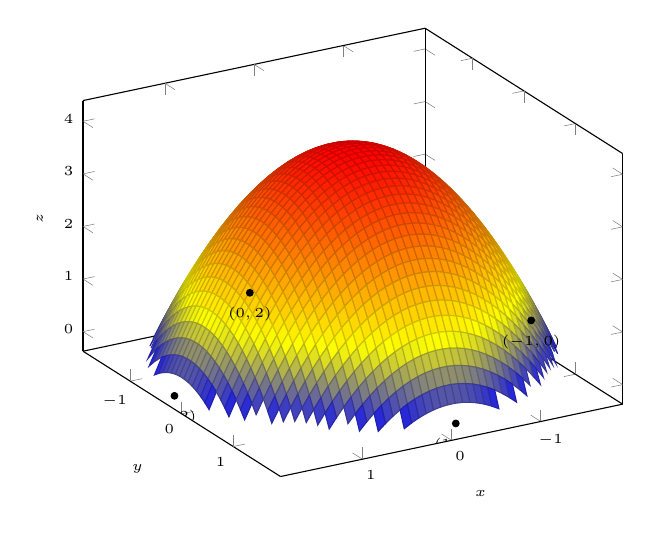
\begin{tikzpicture}
        \begin{axis}[
            view={150}{30},
            xlabel=$x$,
            ylabel=$y$,
            zlabel=$z$,
            domain=-2:2,
            samples=50,
            restrict z to domain=0:4,
            xtick={-2,-1,0,1,2},
            ytick={-2,-1,0,1,2},
            ztick={0,1,2,3,4},
            every axis/.append style={font=\tiny},
        ]
            \addplot3[surf] {4-x^2-y^2};
            \node[label={270:{$(1,1)$}},circle,fill,inner sep=1pt] at (axis cs:0,2,0) {};
            \node[label={270:{$(0,2)$}},circle,fill,inner sep=1pt] at (axis cs:2,0,0) {};
            \node[label={270:{$(-1,0)$}},circle,fill,inner sep=1pt] at (axis cs:-2,0,0) {};
             \node[label={270:{$(0,2)$}},circle,fill,inner sep=1pt] at (axis cs:0,-2,0) {};
        \end{axis}
\end{tikzpicture}

\end{center}
    
In order for us to compute the surface integral in the following theorem that can be found in the textbook which states:

\textbf{Theorem.} Let $C$ be a smooth curve given by the vector function $\mathbf{r(t)}$, $a<t<b$. Let $f$ be a differentiable function of two or three variables whose gradient vector $\nabla f$ is continuous on $C$. 

\begin{equation}
    \int_S \Delta \times \mathbf{F} \cdot d\mathbf{S} = \int_a^b \mathbf{F}(\mathbf{r}(t)) \cdot \mathbf{r}'(t) dt
\end{equation}

Looking at the formula, I began by finding what our $\mathbf{r}(t))$ is, Then, I began by observing/solving the surface on the -XY- Plane, where $z = 0$


\begin{align*}
z = 4 - x^2 - y^2 \\
\text{when z = 0: } \\
x^2 + y^2 = 4 \\
\end{align*}

\begin{center}
  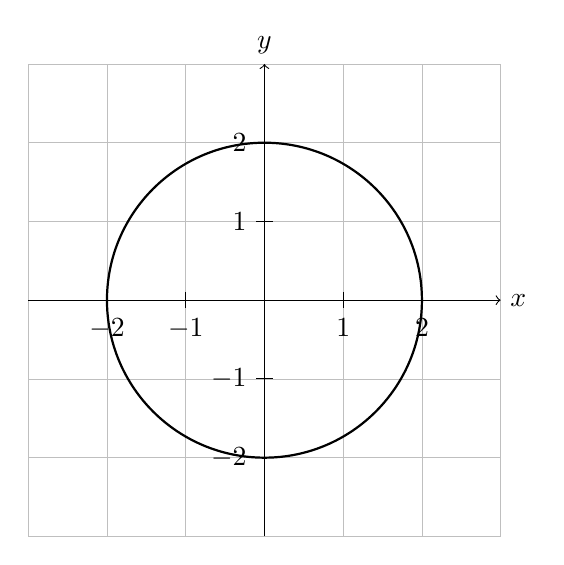
\begin{tikzpicture}
    \draw[step=1cm,gray!50,very thin] (-3,-3) grid (3,3); % grid
    \draw[->] (-3,0) -- (3,0) node[right] {$x$}; % x-axis
    \draw[->] (0,-3) -- (0,3) node[above] {$y$}; % y-axis
    \foreach \x in {-2,-1,1,2}
        \draw (\x cm,3pt) -- (\x cm,-3pt) node[below] {$\x$}; % labels on x-axis
    \foreach \y in {-2,-1,1,2}
        \draw (3pt,\y cm) -- (-3pt,\y cm) node[left] {$\y$}; % labels on y-axis
    \draw[thick] (0,0) circle [radius=2]; % circle
  \end{tikzpicture}
\end{center}

From this point on I figured that using polar coordinates can be very useful. I began by finding the polar coordinates for $x^2 + y^2 = 4$
and by viewing the graph, we can see that the radius $= 2$. To which we can solve the following

\begin{alignat}{2}
    x &= 2\cos(\theta) \quad && \\
    y &= 2\sin(\theta) \quad && \\
    r(t) &= 2\cos(\theta) + 2\sin(\theta) \quad && \\
    r'(t) &= -2\sin(\theta) + 2\cos(\theta) \quad && \\
    \vec{F}(r(t)) &= \langle 2\cos(\theta), 2\sin(\theta), 2\cos(\theta) \cdot 2\sin(\theta) \cdot 0 \rangle. \\
    &= \langle 2\cos(\theta), 4\sin^2(\theta), 0 \rangle \quad && \\
    \vec{F}(r(t)) \cdot r'(t) &= \langle -4\cos(\theta) \cdot \sin(\theta) + 8\sin^2(\theta) \cdot \cos(\theta) \rangle \quad &&
\end{alignat}

I can now begin by solving the following equation:

\begin{alignat}{2}
    &= \int_0^{2\pi} \mathbf{F}(\mathbf{r}(t)) \cdot \mathbf{r}'(t) dt && \\
    &= \int_0^{2\pi} (-4\cos(\theta) \sin(\theta) + 8\sin^2(\theta) \cos(\theta)) d\theta && \\
    &= -4\int_0^{2\pi} \cos(\theta) \cdot \sin(\theta) d\theta + 8\int_0^{2\pi} \sin^2(\theta) \cdot \cos(\theta) d\theta && \\
    &= -4\int_0^{2\pi} u \cdot d(\sin(\theta)) + 8\int_0^{2\pi} u^2 \cdot d(\sin(\theta)) && \text{where } u = \sin(\theta) \\
    &= -4\int_0^{2\pi} d(\cos(\theta)) + 8\int_0^{2\pi} (1 - \cos^2(\theta)) d(\cos(\theta)) && \text{substitute } d(\sin(\theta)) = \cos(\theta) d\theta \\
    &= -4[sin(\theta)]_0^{2\pi} + 8[\frac{1}{3}(sin^3\theta)]_0^{2\pi} && \\
    &= -4(0 - 0) + 8(0 - 0) \\
    &= 0
\end{alignat}

Hence, by using the line integral, and evaluating directly I got:

\begin{center}
    \textbf{Surface Integral = } 0
\end{center}

\section{Part 2: Applying Stokes’ Theorem (Computing the Line Integral)}

In-order to apply Stokes' Theorem to calculate the line integral, I will be using the following formula:


\textbf{Theorem.} Let $S$ be an oriented piecewise-smooth surface that is bounded by a simple, closed, piecewise-smooth boundary curve C with positive orientation. Let $\vec{F}$ be a vector field whose components have continuous partial derivatives on an open region in $\mathbb{R^3}$  that contains S.

\begin{equation}
    \int_C \mathbf{F} \cdot d\mathbf{r} = \int \int_D curl \text{\textbf{F}} \cdot d\textbf{S} 
\end{equation}

As mentioned above, I will begin by evaluating the \textbf{curl} of the vector field, using the vector field we were given \textbf{\vec{F} = $\langle x,y^2,xyz \rangle$}
 \\ 
 
\textbf{Lets let}: \\
\textbf{P(x,y,z) = x} \\
\textbf{Q(x,y,z) = $\textbf{y^2}$} \\
\textbf{R(x,y,z) = xyz} 

\begin{align}
    \text{\textbf{curl }}\vec{F}\text{\textbf{ = }}
    \begin{pmatrix}
        \vec{i} & \vec{j} & \vec{k} \\
        \frac{\partial}{\partial x} &   \frac{\partial}{\partial y} &   \frac{\partial}{\partial z} \\
        P & Q & R 
    \end{pmatrix}
    =
    \begin{vmatrix}
         \frac{\partial}{\partial y} & \frac{\partial}{\partial z} \\
         Q & R 
    \end{vmatrix}
    \vec{i} - 
    \begin{vmatrix}
         \frac{\partial}{\partial x} & \frac{\partial}{\partial z} \\
         P & R 
    \end{vmatrix}
    \vec{j} +
     \begin{vmatrix}
         \frac{\partial}{\partial x} & \frac{\partial}{\partial y} \\
         P & Q 
    \end{vmatrix}
    \vec{k} 
\end{align}

Hence, curl = $\mathbf{\nabla \times F = \langle xz, -yz, 0 \rangle}$
\\ 
\\

Now that we know our curl, we can begin by expressing the surface S in terms of cylindrical coordinates:

\begin{align}
    S(p, \theta) = \left\{
                \begin{aligned}
                    \textbf{x} &= p\cos(\theta) \\
                    \textbf{y} &= p\sin(\theta) \\
                    \textbf{z} &= 4 - p^2
                \end{aligned}
                \right.
\end{align}

Now we will perform the calculation of the fundamental vector product:
Using the following theorem:

\textbf{Theorem.} If $S$ is a smooth orientable surface given in parametric form by a vector function $r(u,v)$, then it is automatically supplied with the orientation of the unit normal vector.

The unit normal vector is given by

\begin{equation}
    n = \frac{\textbf{r}_u \times \textbf{r}_v}{|\textbf{r}_u \times \textbf{r}_v|}
\end{equation}

where $\textbf{r}_u$ and $\textbf{r}_v$ are the partial derivatives of $\textbf{r}$ with respect to $u$ and $v$, respectively.

Applying this theorem to our problem, I will begin by defining the following:

\begin{align}
    \text{\textbf{curl }}\vec{F}\text{\textbf{ = }}
    \begin{pmatrix}
        \vec{i} & \vec{j} & \vec{k} \\
        \frac{\partial}{\partial x} &   \frac{\partial}{\partial y} &   \frac{\partial}{\partial z} \\
        P & Q & R 
    \end{pmatrix}
    =
    \begin{vmatrix}
         \frac{\partial}{\partial y} & \frac{\partial}{\partial z} \\
         Q & R 
    \end{vmatrix}
    \vec{i} - 
    \begin{vmatrix}
         \frac{\partial}{\partial x} & \frac{\partial}{\partial z} \\
         P & R 
    \end{vmatrix}
    \vec{j} +
     \begin{vmatrix}
         \frac{\partial}{\partial x} & \frac{\partial}{\partial y} \\
         P & Q 
    \end{vmatrix}
    \vec{k} 
\end{align}


\begin{align}
    &= (2p^2cos(\theta))\vec{i} + (2p^2sin(\theta))\vec{j} + p(cos^2(\theta)) + psin^2(\theta))\vec{k} \\
    &= (2p^2cos(\theta))\vec{i} + (2p^2sin(\theta))\vec{j} + p(cos^2(\theta) + sin^2(\theta))\vec{k} \\
    &= (2p^2cos(\theta))\vec{i} + (2p^2sin(\theta))\vec{j} + (p)\vec{k} \\
\end{align}

Now that I have successfully completed the fundamental vector product, I will calculate the line integral by using the following formula:

\begin{equation}
    \text{\textbf{I}}s = \iint \operatorname{curl}(\vec{F} ) \cdot (S_p \times S_\theta) d\theta dp,
\end{equation}

Here, I will compute: $$\operatorname{curl}(\vec{F} ) \cdot (S_p \times S_\theta)$$

\begin{align}
    \begin{split}
    &\langle xz, -y, 0 \rangle \cdot \langle 2p^2\cos(\theta), 2p^2\sin(\theta), p \rangle \\
    &= 2xzp^2\cos(\theta) - 2yzp^2\sin(\theta) + 0 \\
    &= 2p^2(xz\cos(\theta) - yz\sin(\theta)) + 0 \\
    &= 2p^2[(p\cos(\theta))(4-p^2)]\cos(\theta) - 2p^2[(p\sin(\theta))(4 - p^2)]\sin(\theta) \\
    &= 2p^2[4p\cos(\theta)-p^3\cos(\theta)]\cos(\theta) - 2p^2[4p\sin(\theta) - p^3\sin(\theta)]\sin(\theta) \\
    &= 2p^2[4p\cos^2(\theta)-p^3cos^2(\theta)] - 2p^2[4p\sin^2(\theta) - p^3\sin^2(\theta)]\\
    &= 2p^2[4p(cos^2(\theta)-sin^2(\theta) - p^3(cos^2(\theta) - sin^2(\theta)] \\
    &= 8p^3cos(2\theta) - 2p^5cos(2\theta)
    \end{split}
\end{align}


\begin{align}
    \text{\textbf{I}}_s &=\int_0^{2} 8p^3 \int_0^{2\pi}cos(2\theta) d\theta - 2p^5 \int_0^{2\pi}cos(2\theta) d\theta dp \\
    &= \int_0^2 4p^3[sin(2(2\pi)) - sin(2(2(0)))] - p^5 [sin(2(2\pi)) - sin(2(2(0)))\\
    &= \int_0^2 4p^3[0-0] \\
    &= \int_0^2 0 dp \\
    = 0 \\ 
\end{align}

\begin{align}
    \textbf{Hence, by using Stokes' theorem, I got a surface integral of 0}
\end{align}

\section{Part 3: Applying Stokes’ Theorem (Computing the new Surface Integral)}

For this portion of the project, I will begin by applying the Stokes\' Theorem to a triangle will the vertices \textbf{(1,0,0), (0,1,0), (0,0,2)}.

\begin{figure}
  \centering
  \includegraphics[width=0.5\textwidth]{three.png}
  \caption{Triangle with vertices: (1,0,0), (0,1,0), (0,0,2)}
  \label{fig:example}
\end{figure}


We know by viewing the graph that our equation for the plane is:

\begin{equation}
    z = 2 \text{ - } 2x \text{ - } 2y
\end{equation}

I will use the formula that I used above:

\begin{equation}
    &= \int_0^2 \int_0^1 curl \biggl(\vec{F} \cdot \frac{r_u \times r_v}{|r_u \times r_v|}\biggr) &
\end{equation}

\begin{center}
    Using the curl from above, we get:
\end{center}

\begin{equation}
    curl(\vec{F} = (xz)\vec{i} - (yz)\vec{j} + 0
\end{equation}

\begin{center}
    Solving $r_u \times r_v$, we get: $r_u \times r_v = 2\vec{i} + 2\vec{j} + \vec{k}$ \\
\end{center}

\begin{align}
\int_C F dr &= \int_0^1 \int_0^{1-x} (2x+4(2-2x-2y)-2y) dy dx \\
&= \int_0^1 \int_0^{1-x} (-6x-10y+8) dy dx \\
&= \int_0^1 (-3x^2-5x+4) dx \\
&= \frac{4}{3}\\
\end{align}
\textbf{Hence, similarly to how I used part two of this project. I was able to find the surface integral!}


\section{Part 4: Conclusions}

\textbf{Q: Check the values of the three integrals you computed in this project.  How do they compare? What does this say about the relationship between the vector field, surface, and curve in terms of the answers you calculated?}

There is a strong relationship between the vector field, surface, and curve. Specifically, the fact that the integral values in parts one and two were 0 suggests that the vector field is divergence-free over the surface, meaning that there is no net flow of the vector field across the surface. This is consistent with the fact that the surface in parts one and two was a closed surface, i.e., one that encloses a volume.

In contrast, the non-zero value of the integral in part three indicates that the vector field is not divergence-free over the curve, meaning that there is a net flow of the vector field across the curve. This is consistent with the fact that the curve in part three was an open curve, i.e., one that does not enclose a volume.

Overall, the values of the integrals provide insight into the behavior of the vector field over the surface and curve, and demonstrate the intimate relationship between the vector field, surface, and curve in terms of their flux and circulation properties.
 
\textbf{Q: Do the numbers you found make sense in light of Stokes’ Theorem and what it states?  Why or why not?}

Initially, I was perplexed by the repeated value of 0 for the surface integral in the first part of the project. However, upon reflection, I realized that this outcome was reasonable. This is because we were only examining the portion of the paraboloid where z is greater than or equal to 0. Given that the paraboloid is symmetrical in shape, it follows that the surface integral would indeed evaluate to 0. Since every point on the surface of the paraboloid will always have a positive and negative point!


\textbf{Q: Which of the three integrals was easiest to compute?  Why?  
Sometimes Stokes’ Theorem is used to “change the surface” of integration.  What do you think this means in light of the work you did in this project?}

In my view, the easiest task in the project was computing the surface integral in part one. This is because I have more experience evaluating integrals on the XY plane and using polar coordinates. Furthermore, I found this approach more intuitive than using Stokes' theorem.
\\
However, in parts two and three, where I had to use Stokes' theorem, I found it much simpler to "simplify" the equations. Depending on the complexity of the surface, I would prefer using Stokes' theorem to evaluate it because it uses the curl of the vector field, which provides information about the behavior of the vector field over the surface and its boundary curve. This can simplify the computation of surface integrals, making it a valuable tool in various fields.
\end{document}
